\RequirePackage{fix-cm}
\documentclass[a5paper]{ltjsarticle}
\usepackage{amsmath}
\usepackage{amssymb}
\usepackage{ascmac}
\usepackage{thedarkness}
\RequirePackage{geometry}
\newlength\nzw{\normalsize\global\nzw1\ZW\relax}
\geometry{nohead,top=18mm,bottom=17mm}
\geometry{textwidth=40\nzw}
\topskip10pt
\usepackage{graphicx}
\usepackage{wrapfig}
\usepackage{multicol}
\usepackage{thedarkness}
\usepackage{siunitx}
\usepackage{bm}
\usepackage{tikz}
\usetikzlibrary{math,intersections,calc,arrows.meta,patterns,angles}
\usepackage{tikz-3dplot} 
\usepackage{here}
\usepackage{caption}
\usepackage{color}
\renewcommand{\columnseprule}{0.4pt}
\newcommand{\bhline}{\noalign{\hrule height 1.5pt}}
\newcommand{\bvline}{\vrule width 1.5pt}
\newcommand{\pie}[1]{\tikz[baseline=-3pt]{\draw[thick](0,0)circle(0.4);\filldraw[pattern=north east lines]((0,0.4)arc(90:#1:0.4)--(0,0)--cycle;)}}%chktex 36 
\newcommand{\minitet}[3]{
  \begin{tikzpicture}[baseline=-3pt,tdplot_main_coords,scale=0.3]
    \tikzmath{\a=1;}
    \tikzmath{\b=2*sqrt(6)*\a;}
    \coordinate (I) at (0,0,{\a});
    \coordinate (A) at ({\b/sqrt(3)},0,0);
    \coordinate (B) at ({-sqrt(3)*\b/6},{\b/2},0);
    \coordinate (C) at ({-sqrt(3)*\b/6},{-\b/2},0);

    \draw(I)node[above left]{I};
    \draw(A)node[left]{#1};
    \draw(B)node[below]{#2};
    \draw(C)node[right]{#3};
    \draw(A)--(B)--(C)
    (A)--(I)--(B) (I)--(C);
    \draw[dashed](A)--(C);
  \end{tikzpicture}
}
\newcommand{\floattxt}[1]{{\fboxsep=0.1ex\colorbox{white}{#1}}}
\begin{document}
\tableofcontents
\clearpage

\section{小学生コース}
\subsection*{問1 物理室}
\begin{itembox}[l]{問題}
  とある学校にはA棟とB棟があり,両棟合わせて54教室あります。
  A棟はB棟よりも4教室多いです。また,B棟の特別教室の数はB棟の24\% を占めます。 B棟の特別教室は何室あるか答えなさい。
\end{itembox}

まずは,A棟の教室数を$a$,B等の教室数を$b$とおきます。すると,
\begin{align}
  a+b=54\label{sum}\\
  a=b+4\label{def}
\end{align}
と書けます。\eqref{def}を\eqref{sum}に代入して,
\begin{align*}
  (b+4)+b&=54\\
  2b+&=54-4\\
  b&=25
\end{align*}
よって,B棟の教室数は25棟とわかりました。B棟の特別教室はこの24\% なので,
\[25\times \frac{24}{100}=6 \qquad \text{\underline{答え. 6室}}\]


\subsection*{問2 化学室}
\begin{itembox}[l]{問題}
  \centering
  $\displaystyle\dwide 0,\, 1,\, \frac{5}{3},\, 1\frac{2}{9},\, \text{1割2分}$\\
  大きい順に並べましょう。
\end{itembox}

このままでは比べられないので,小数に変換しましょう。\\
$\displaystyle\dwide \frac{5}{3}=1.66\ldots ,\: 1\frac{2}{9}=1.22\ldots ,\: \text{1割2分}=1.2$ なので,
\begin{center}
\begin{tabular}{c|c|c|c|c}%chktex 44
  0&1&$\displaystyle  \frac{5}{3}$&$\displaystyle  1\frac{2}{9}$&1割2分\\
  0&1&1.66\ldots&1.22\ldots&1.2
\end{tabular}
\end{center}
このように対応します。よって答えは,\\
\centerline{\underline{$\displaystyle\frac{5}{3}$, $\displaystyle\dwide 1\frac{2}{9}$, 1割2分, 1, 0}}

\subsection*{問3 生物室}
\begin{itembox}[l]{問題}
  時刻が9月10日深夜1時20分です。
  30分前は,何時何分でしょう。
\end{itembox}

9月10日深夜1時20分の20分前は9月10日深夜1時00分になります。
そこからさらに10分前は9月10日深夜0時50分です。
よって, \underline{答え. 0時50分}


\subsection*{問4 特別棟4階}
\begin{itembox}[l]{問題}
  \[1,2,2,3,3,3,4,4,4,4,\cdots\]
  上の数列はある規則に沿って並んでいます。
  30番目の数はいくつでしょう。
\end{itembox}

この数列は,数字がその数字の数だけ並んで続いていきます。よって書き出すと,
\begin{align*}
  1,2,2,3,3,3,4,4,4,4,\\
  5,5,5,5,5,6,6,6,6,6,\\
  6,7,7,7,7,7,7,7,8,8
\end{align*}
となるので, \underline{答え. 8}


\subsection*{問5 昇降口}
\begin{itembox}[l]{問題}
\begin{wrapfigure}{r}{60mm}
  \vspace{-10mm}
  \centering
  {\renewcommand{\arraystretch}{2}
  \begin{tabular}{ccc}
    & Aさん & Bさん\\
  チョコケーキ &\pie{-90} $\dfrac{1}{2}$ & \pie{-180} $\dfrac{3}{4}$\\
  イチゴケーキ &\pie{-180} $\dfrac{3}{4}$ & \pie{40} $\dfrac{1}{9}$\\
  ホットケーキ &\pie{-126} $\dfrac{3}{5}$ & \tikz[baseline=-3pt]{\filldraw[thick,pattern=north east lines](0,0)circle(0.4);}\pie{54} $\dfrac{11}{10}$
  \end{tabular}
  }
\end{wrapfigure}
AさんとBさんの取ったケーキの分量の差はいくらでしょう。
ただし,ケーキの大きさはどの種類も同じとします。
\vspace{15mm}
\end{itembox}

通分して,分数の足し算・引き算をしましょう。
\begin{multicols}{2}
Aさん
\begin{align*}
  &\frac{1}{2}+\frac{3}{4}+\frac{3}{5}\\
  =&\frac{10}{20}+\frac{15}{20}+\frac{12}{20}\\
  =&\frac{37}{20}
\end{align*}

Bさん
\begin{align*}
  &\frac{3}{4}+\frac{1}{9}+\frac{11}{10}\\
  =&\frac{135}{180}+\frac{20}{180}+\frac{198}{180}\\
  =&\frac{353}{180}
\end{align*}
\end{multicols}
2人の分量の差は,
\begin{align*}
  &\frac{353}{180}-\frac{37}{20}\\
  =&\frac{353}{180}-\frac{333}{180}\\
  =&\frac{20}{180}\\
  =&\frac{1}{9}\qquad \underline{\text{答え.}\: \frac{1}{9} }
\end{align*}


\subsection*{問6 セミナーハウス}
\begin{itembox}[l]{問題}
  A空港とB空港の間は5100 km 離れています。
  その間を時速 900 km の飛行機で移動すると,
  何時間何分かかるでしょう。
\end{itembox}

距離と速さがわかっていて,時間を求める問題です。
「み・は・じ」\footnote{\scalebox{2}{\textcircled{\raisebox{0.35ex}{\scalebox{0.44}{$\frac{\text{み}}{\: \text{は|じ}\: }$}}}}。「き・は・じ」や「は・じ・き」と言ったりもする。}を使って解くと,
\[\frac{5100}{900}=\frac{17}{3}=5+\frac{2}{3} \quad [\text{時間}]\]
$\displaystyle \frac{2}{3}$ 時間は40分なので,\qquad
\underline{答え. 5時間40分}


\subsection*{問7 体育館}
\begin{itembox}[l]{問題}
  \centering
  斜線部の面積を求めましょう。\\\vspace{2ex}
  \begin{tikzpicture}[scale=0.3]
    \begin{scope}\clip(-2.5,-2)rectangle(10,7);
    \tikzmath{\r=(sqrt(89))/2;}
    \coordinate(A) at (0,5);
    \coordinate(B) at (0,0);
    \coordinate(C) at (8,0);
    \coordinate(P) at (4,0);
    \draw(B) to[out=150,in=210, edge node={node [midway,fill=white]{\SI{5}{cm}}}] (A);
    \draw(P) to[out=315,in=225, edge node={node [midway,fill=white]{\SI{4}{cm}}}] (C);
    \path[name path=C1](4,2.5)circle(\r);
    \path[name path=C2](C)circle(7);
    \path[name path=C3](A)circle(2);
    \path[name intersections={of= C1 and C2, by={D,null}}];
    \draw[thick,name path=line](A)--(B)--(C)--(D)--cycle;
    \path[name intersections={of= line and C3, by={null,Q}}];
    \filldraw[thick,pattern=north east lines](A)--(P)--(C)--(Q)--cycle;
    \draw pic[draw=black, angle radius=0.2cm]{right angle=C--B--A};
    \draw pic[draw=black, angle radius=0.2cm]{right angle=C--D--A};
    \draw(A) to[out=76,in=136, edge node={node [above]{\SI{2}{cm}}}] (Q);
    \draw(C) to[out=46,in=346, edge node={node [midway,fill=white]{\SI{7}{cm}}}] (D);
    \end{scope}
    \end{tikzpicture}    
\end{itembox}

\begin{wrapfigure}{r}{40mm}
  \begin{tikzpicture}[scale=0.3]
    \begin{scope}\clip(-2.5,-2)rectangle(10,7);
    \tikzmath{\r=(sqrt(89))/2;}
    \coordinate(A) at (0,5);
    \coordinate(B) at (0,0);
    \coordinate(C) at (8,0);
    \coordinate(P) at (4,0);
    \draw(B) to[out=150,in=210, edge node={node [midway,fill=white]{\SI{5}{cm}}}] (A);
    \draw(P) to[out=315,in=225, edge node={node [midway,fill=white]{\SI{4}{cm}}}] (C);
    \path[name path=C1](4,2.5)circle(\r);
    \path[name path=C2](C)circle(7);
    \path[name path=C3](A)circle(2);
    \path[name intersections={of= C1 and C2, by={D,null}}];
    \draw[thick,name path=line](A)--(B)--(C)--(D)--cycle;
    \path[name intersections={of= line and C3, by={null,Q}}];
    \draw[thick,pattern=north east lines](A)--(P)--(C)--(Q)--cycle;
    \draw[thick](A)--(C);
    \draw pic[draw=black, angle radius=0.2cm]{right angle=C--B--A};
    \draw pic[draw=black, angle radius=0.2cm]{right angle=C--D--A};
    \draw(A) to[out=76,in=136, edge node={node [above]{\SI{2}{cm}}}] (Q);
    \draw(C) to[out=46,in=346, edge node={node [midway,fill=white]{\SI{7}{cm}}}] (D);
    \end{scope}
    \end{tikzpicture}    
\end{wrapfigure}
右の図のように補助線を引きます。
すると,底辺が2,高さが7の三角形と底辺が4,高さが5の三角形に分けることができます。
よって面積は,
\begin{align*}
  2\times 7\div 2+4\times 5\div 2&=7+10\\
  &=17
\end{align*}
\underline{答え. \SI{17}{cm^2}}


\subsection*{問8 本部前}
\begin{itembox}[l]{問題}
  \centering
  斜線部の面積を求めましょう。ただし,円周率は3.14とする。
  \begin{tikzpicture}[scale=0.5]
    \filldraw[pattern=north east lines,thick](0,0)arc(270:360:4)arc(180:270:4)--cycle;
    \coordinate(A) at (0,0);
    \coordinate(B) at (0,4);
    \coordinate(P) at (4,4);
    \coordinate(C) at (8,4);
    \draw(A)to[out=135,in=225, edge node={node [midway,fill=white]{\SI{4}{cm}}}](B);
    \draw(B)to[out=45,in=135, edge node={node [midway,fill=white]{\SI{4}{cm}}}](P);
    \draw(P)to[out=45,in=135, edge node={node [midway,fill=white]{\SI{4}{cm}}}](C);
    \draw[thick](0,0)rectangle(8,4);
  \end{tikzpicture}
\end{itembox}

斜線部の面積は,\SI{4}{cm}\times\SI{8}{cm}の長方形から半径\SI{4}{cm}の半円を引いたものに等しいので,
\[4\times 8-4\times 4\times 3.14 \div 2 =32-25.12=6.88\]
\underline{答え. \SI{6.88}{cm^2}}


\subsection*{問9 水道前}
\begin{itembox}[l]{問題}
  仕入れた状態で300円の洋服を20\% の利益をつけて売りたい。 
  この洋服を何円で売ればよいだろうか。
\end{itembox}

300円の洋服に20\% の利益をつけるので,利益は$\displaystyle\dwide 300\times \frac{20}{100}=60$円。\\
売値は原価+利益なので,$300+60=360$\qquad \underline{答え. 360円}


\subsection*{問10 屋上入口}
\begin{itembox}[l]{問題}
  \centering
  次の立体の体積を求めましょう。\vspace{2ex}
  \tdplotsetmaincoords{70}{20}
  \begin{tikzpicture}[tdplot_main_coords,scale=0.7]
    \tikzmath{\x=2.55;}
    \coordinate (A) at (0,0,0);
    \coordinate (B) at (0,0,5);
    \coordinate (C) at (2,0,5);
    \coordinate (D) at (2,0,2);
    \coordinate (E) at (4,0,2);
    \coordinate (F) at (4,0,5);
    \coordinate (G) at (8,0,5);
    \coordinate (H) at (8,0,0);

    \coordinate (I) at (0,4,0);
    \coordinate (J) at (0,4,5);
    \coordinate (K) at (2,4,5);
    \coordinate (L) at (2,4,2);
    \coordinate (M) at (4,4,2);
    \coordinate (N) at (4,4,5);
    \coordinate (O) at (8,4,5);
    \coordinate (P) at (8,4,0);
    \coordinate (LM) at (\x,4,2);
    \draw(A) to[out=135,in=225,edge node={node [midway,fill=white]{\SI{5}{cm}}}] (B);
    \draw(A) to[out=323,in=203,edge node={node [midway,fill=white]{\SI{8}{cm}}}] (H);
    \draw(H) to[out=0,in=270,edge node={node [midway,fill=white]{\SI{4}{cm}}}] (P);
    \draw[thick,dashed]
      (A)--(I)--(P)
      (N)--(M)--(E)
      (LM)--(M)
      (I)--(J);
    \draw(D) to[out=45,in=315,edge node={node [midway,fill=white]{\SI{3}{cm}}}] (C);
    \draw(D) to[out=308,in=218,edge node={node [midway,fill=white]{\SI{2}{cm}}}] (E);
    \draw[thick] 
      (A)--(B)--(C)--(D)--(E)--(F)--(G)--(H)--cycle
      (B)--(J)--(K)--(C)
      (G)--(O)
      (H)--(P)--(O)--(N)--(F)
      (D)--(L)--(K)
      (L)--(LM);
  \end{tikzpicture}
\end{itembox}

このような立体の体積は底面積\times 高さで求めることができます(同じ形の板がたくさん重なっているイメージ)。%chktex 1
この問題では底面は手前に向いている面です。\\
底面積は$5\times 8$の長方形から$2\times 3$の長方形を引いたものなので,
\begin{align*}
  (5\times 8-2\times 3)\times 4&=34\times 4\\
  &=136
\end{align*}
\underline{答え. \SI{136}{cm^3}}


\subsection*{問11 徘徊者}
\begin{itembox}[l]{問題}
  81をある1より大きい整数で割ると,小数の部分のどこかに1995という数の並びが現れました。
  このような整数のうち,最も小さいものを求めましょう。
\end{itembox}

求める数を$x$とおきます。$\displaystyle \frac{81}{x}=\cdots . \cdots 1995\cdots $\\
小数を$10,100$倍していくと小数点を右にずらせる。
さらに整数部分を引くと,
\[\frac{a}{x}=0.1995\cdots (\text{$a$は1以上の整数})\]
まず,これを満たす$x$を見つける。\\
\[0.1995\leqq \frac{a}{x}\leqq 0.1996\]
5倍して,1から引くと,
\[0.002\leqq \frac{b}{x}\leqq 0.0025\quad (b=x-a)\]
これを変形して,
\[400b \leqq x \leqq 500b\]
このとき,$x$の最小値を求めればいいので,$b=1$の時を考える。\\
$x=400$のとき,$0.205$となる。\\
$x=401$のとき,$0.201995\cdots$となり,条件を満たす。
よって \underline{答え. 401}


\section{中学生コース}
\subsection*{問1 物理室}
\begin{itembox}[l]{問題}
  $-2^2$を計算しなさい。
\end{itembox}

指数の2は$-2$の中の2のみにかかっているので,答えは
\begin{align*}
  -2^2&=-(2^2)\\
&=-(2\times2)\\
&=\mathbf{-4}
\end{align*}

ちなみに${(-2)}^2$の指数2は,$(-2)$全体にかかっているので,
\begin{align*}
  {(-2)}^2&=(-2)\times2\\
&=4
\end{align*}


\subsection*{問2 化学室}
\begin{itembox}[l]{問題}
  次の中で関数 $y=x$のグラフとして最も適するものを①\textasciitilde ④の中から一つ選びなさい。\\%chktex 1
  \begin{center}
    \begin{tabular}{cc}
      ①
      \begin{tikzpicture}[baseline=30pt,>=stealth,scale=0.6]
      \draw[->](-2,0)--(2,0)node[above]{$x$};
      \draw[->](0,-2)--(0,2)node[left]{$y$};
      \draw(0,0)node[below left]{O};
      \draw[thick](-2,1)--(2,1);
      \end{tikzpicture}&
      ②
      \begin{tikzpicture}[baseline=30pt,>=stealth,scale=0.6]
      \draw[->](-2,0)--(2,0)node[above]{$x$};
      \draw[->](0,-2)--(0,2)node[left]{$y$};
      \draw(0,0)node[below left]{O};
      \draw[thick](1,-2)--(1,2);
      \end{tikzpicture}\\
      ③
      \begin{tikzpicture}[baseline=30pt,>=stealth,scale=0.6]
      \draw[->](-2,0)--(2,0)node[above]{$x$};
      \draw[->](0,-2)--(0,2)node[left]{$y$};
      \draw(0,0)node[below right]{O};
      \draw[thick](-2,-2)--(2,2);
      \end{tikzpicture}&
      ④
      \begin{tikzpicture}[baseline=30pt,>=stealth,scale=0.6]
      \draw[->](-2,0)--(2,0)node[above]{$x$};
      \draw[->](0,-2)--(0,2)node[left]{$y$};
      \draw(0,0)node[below left]{O};
      \draw[thick](-2,2)--(2,-2);
      \end{tikzpicture}
      \end{tabular}
  \end{center}
\end{itembox}

\subsubsection*{解法① 表を作って考える}
\begin{table}[h]
  \centering
  \begin{tabular}{|c||c|c|c|c|c|c|c|}%chktex 44
    \hline%chktex 44
     $x$ & -3 & -2 & -1 & 0 & 1 & 2 & 3 \\ 
     \hline%chktex 44
     $y$ & -3 & -2 & -1 & 0 & 1 & 2 & 3 \\ 
     \hline%chktex 44
  \end{tabular}
\end{table}
これらの点を通るのは,{\bfseries③}のグラフ。

\subsubsection*{解法② $y=x$のグラフはどのようなグラフになるのか考える}
$y=x$は比例定数1の比例の関係になっている。
比例のグラフは原点を通る直線なので,条件を満たすのは{\bfseries③}のグラフ。


\subsection*{問3 生物室}
\begin{itembox}[l]{問題}
  次のデータは,生徒8人のテストの結果を得点が低い順に並べたものである。
  このとき,中央値(メジアン)の値を求めなさい。
  \begin{center}
  \begin{tabular}{|c||c|c|c|c|c|c|c|c|c|} \hline%chktex 44
     No. & 1 & 2 & 3 & 4 & 5 & 6 & 7 & 8  \\ \hline%chktex 44
     得点 & 53 & 57 & 65 & 66 & 68 & 69 & 78 & 82 \\ \hline%chktex 44
  \end{tabular}
\end{center}
\end{itembox}

中央値(メジアン)はデータを小さい順に並べたものの中で真ん中にあたるものです。
データの数は偶数で真ん中が2つ出てくるので,2つの値(得点)の平均を取ります。\\
よって,$\displaystyle\dwide \frac{66+68}{2}=\mathbf{67}$点となります。


\subsection*{問4 特別棟4F}
\begin{itembox}[l]{問題}
  大小2つのサイコロをそれぞれ1回振るとき,出目の積が偶数になる確率を求めなさい。
  ただし,サイコロの出目は同様に確からしいものとする。
\end{itembox}

サイコロを2個振る問題は$6\times6$の表を使って考えます。表を作ると,
\begin{table}[H]
  \centering
  \begin{tabular}{|c||c|c|c|c|c|c|c|}%chktex 44
    \hline%chktex 44
      & 1 & 2 & 3 & 4 & 5 & 6 \\
    \bhline%
    1 & 1 & 2 & 3 & 4 & 5 & 6 \\
    \hline%chktex 44
    2 & 2 & 4 & 6 & 8 & 10 & 12 \\
    \hline%chktex 44
    3 & 3 & 6 & 9 & 12 & 15 & 18 \\
    \hline%chktex 44
    4 & 4 & 8 & 12 & 16 & 20 & 24 \\
    \hline%chktex 44
    5 & 5 & 10 & 15 & 20 & 25 & 30 \\
    \hline%chktex 44
    6 & 6 & 12 & 18 & 24 & 30 & 36 \\
    \hline  %chktex 44
  \end{tabular}
\end{table}
\noindent となり,この中で偶数は27つあるので,求める確率は,$\displaystyle \frac{27}{36}=\mathbf{\frac{3}{4}}$となります。


\subsection*{問5 昇降口}
\begin{itembox}[l]{問題}
  次のヒストグラム(柱状図)と同じデータを用いて表された箱ひげ図として最も適するものを①\textasciitilde ④の中から一つ選びなさい。%chktex 1
  \begin{center}
    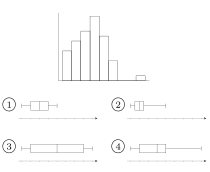
\includegraphics[width=40mm]{./mathclub-f/LV2_Q5.pdf}
  \end{center}
\end{itembox}

箱ひげ図は,最大値,最小値,第\bigcirc 四分位数に注目します。%chktex 1
最大値より,①,②は間違いです。
また,第3四分位数より,③は間違いです。\\
よって,正しい箱ひげ図は{\bfseries ④}です。


\subsection*{問6 セミナーハウス}
\begin{itembox}[l]{問題}
  ${(x-3)}^2=2$を解きなさい。
\end{itembox}

二次方程式の解き方はいくつかありますが,今回は普段使わない平方完成$\left({(x-a)}^p\text{の形にすること}\right)$を使います。
それぞれの根$(\sqrt{\:\:})$をとって,
\begin{align*}
  {(x-3)}^2&=2\\
  x-3&=\pm \sqrt{2}\\
  x&=\bm{3\pm \sqrt{2}}
\end{align*}

平方完成は二次方程式の解の公式の証明に使うので,覚えておくといいかもしれません。


\subsection*{問7 体育館}
\begin{itembox}[l]{問題}
  関数$y=-2x^2$において,$x$の変域が$-2 \leqq x \leqq 1$のとき,$y$の変域を求めなさい。
\end{itembox}

\begin{wrapfigure}{r}{45mm}
  \begin{tikzpicture}[scale=0.5]
    \draw[->,>=stealth,semithick](-2.5,0)--(2,0)node[above]{$x$};
    \draw[->,>=stealth,semithick](0,-9)--(0,1)node[above]{$y$};
    \draw(0,0)node[above right]{O};
    \begin{scope}\clip(-2.5,-9)rectangle(2,1);
      \draw[dashed, domain=-2.5:2]plot(\x, {-2*\x*\x});
      \draw[thick, domain=-2:1]plot(\x, {-2*\x*\x});
    \end{scope}
    \fill(-2,-8)circle(3pt)node[left]{$(-2,-8)$};
    \fill(0,0)circle(3pt)node[above left]{$(0,0)$};
    \fill(1,-2)circle(3pt)node[right]{$(1,-2)$};
  \end{tikzpicture}
  \vspace{-50mm}
\end{wrapfigure}
この問題は,グラフを描いて求めます。実際に描くと,右のようになります。\\
よって,この時の$y$の最大値は$0$,$y$の最小値は$-8$となるので,求める範囲は$\bm{-8 \leqq y \leqq 0}$
\vspace{45mm}


\subsection*{問8 本部前}
\begin{itembox}[l]{問題}
  関数$\displaystyle y=\frac{a}{x}$について,$x$が2から6まで増加するときの$y$の増加量が1であった。
  このとき,$a$の値を求めなさい。
\end{itembox}

この問題では,$a$の値を求める問題なので,$a$に関する方程式を作ります。\\
また,増加量は,増加後の値$-$増加前の値で求められるので,\\
\[\frac{a}{6}-\frac{a}{2}=1\]
という方程式が成り立ちます。この方程式を解いて,$a=\mathbf{-3}$\\


\subsection*{問9 水道前}
\begin{itembox}[l]{問題}
  $\displaystyle \frac{(11^4-2^2)(4^4-1^2)}{(44^2-11^2)+2(4^2-1^2)}$を計算しなさい。
\end{itembox}

このままでも計算できますが,累乗が多くあるので,因数分解,約分を駆使して簡単にすることができます。
特に和と差の積$a^2-b^2=(a+b)(a-b)$が使えることが多いです。
\begin{align*}
  \frac{(11^4-2^2)(4^4-1^2)}{(44^2-11^2)+2(4^2-1^2)}&=\frac{(11^4-2^2)(4^4-1^2)}{11^2(4^2-1^2)+2(4^2-1^2)}\\
  &=\frac{(11^2+2)(11^2-2)(4^2+1)(4^2-1)}{(11^2+2)(4^2-1^2)}\\
  &=(11^2-2)(4^2+1)\\
  &=119\times 17\\
  &=\mathbf{2023}
\end{align*}

この問題では2023を扱った問題でしたが,2023/9/18現在で中3の人は2024,
中2の人は2025\ldots を扱った問題が高校入試で出ると考えられます。
そのため,それぞれの年に対応する素因数分解した形,そして学年ごとに関係なく$11^2$から$20^2$までは覚えておきましょう。


\subsection*{問10 屋上入口}
\begin{itembox}[l]{問題}
  $ \triangle \mathrm{ABC} $ が半径2の円に内接している。
  $ \angle \mathrm{A} =45^{\circ},\, \angle \mathrm{B} =60^{\circ},\, \angle \mathrm{C} =75^{\circ}$ 
  であるとき,$\triangle \mathrm{ABC}$ の面積を求めなさい。
\end{itembox}

円の中心をOとすると,$\mathrm{OB}=\mathrm{OC}=2$なので,$\mathrm{BC}=2\sqrt{2}$\\
Cから垂線CHを引くと,\qquad$\mathrm{BH}=\sqrt{2}$,$\mathrm{CH}=\sqrt{6}$\\
$\mathrm{HC}=\mathrm{AH}$より,\qquad$\mathrm{AH}=\sqrt6$\\
よって,\qquad$\mathrm{AB}=\sqrt{2}+\sqrt{6}$\\
$\triangle \mathrm{ABC}$の面積は\qquad $\displaystyle\dwide \frac{\sqrt{6}(\sqrt{2}+\sqrt{6})}{2}=\bm{3+\sqrt{3}}$


\subsection*{問11 徘徊者}
\begin{itembox}[l]{問題}
  $ \mathrm{AB}=6,\, \mathrm{BC}=10,\, \mathrm{CA}=8$ の$ \triangle \mathrm{ABC}$ がある。
  この三角形の中に大きさの等しい円$ \mathrm{P},\mathrm{Q},\mathrm{R}$ が図のように接しているとき,これらの円の半径を求めよ。
  \begin{center}
    \begin{tikzpicture}[scale=0.4]
      \begin{scope}\clip(-1,-1)rectangle(11,6);
      \tikzmath{\r=10/9;}
      \tikzmath{\x=2;}
      \coordinate(P) at (\x,\r);
      \coordinate(Q) at (\x+2*\r,\r);
      \coordinate(R) at (\x+4*\r,\r);
      \coordinate(B) at (0,0);
      \coordinate(C) at (10,0);
      
      \draw[name path=CP](P)circle(\r);
      \draw(Q)circle(\r);
      \draw[name path=CR](R)circle(\r);
      
      \draw(B)--(C);
      \path[name path=C1](B)circle(\x);
      \path[name path=C2](C)circle(10-\x-4*\r);
      \path[name intersections={of= C1 and CP, by={M,null}}];
      \path[name intersections={of= C2 and CR, by={N,null}}];
      \path[name path=BA](B)--($3*(M)$);
      \path[name path=CA](C)--($3*($(N)-(C)$)+(C)$);
      \path[name intersections={of= BA and CA, by={A}}];
      
      \draw(A)--(B)--(C)--cycle;
      \fill(P)circle(2pt)node[below]{P};
      \fill(Q)circle(2pt)node[below]{Q};
      \fill(R)circle(2pt)node[below]{R};
      \draw(B)node[left]{B};
      \draw(C)node[right]{C};
      \draw(A)node[above]{A};
      \end{scope}
    \end{tikzpicture}
  \end{center}
\end{itembox}

\begin{wrapfigure}{r}{50mm}
  \centering
  \begin{tikzpicture}[scale=0.4]
      \begin{scope}\clip(-1,-1)rectangle(11,6);
      \tikzmath{\r=10/9;}
      \tikzmath{\x=2;}
      \coordinate(P) at (\x,\r);
      \coordinate(Q) at (\x+2*\r,\r);
      \coordinate(R) at (\x+4*\r,\r);
      \coordinate(B) at (0,0);
      \coordinate(C) at (10,0);
      
      \draw[name path=CP](P)circle(\r);
      \draw(Q)circle(\r);
      \draw[name path=CR](R)circle(\r);
      
      \draw(B)--(C);
      \path[name path=C1](B)circle(\x);
      \path[name path=C2](C)circle(10-\x-4*\r);
      \path[name intersections={of= C1 and CP, by={M,null}}];
      \path[name intersections={of= C2 and CR, by={N,null}}];
      \path[name path=BA](B)--($3*(M)$);
      \path[name path=CA](C)--($3*($(N)-(C)$)+(C)$);
      \path[name intersections={of= BA and CA, by={A}}];
      
      \draw(A)--(B)--(C)--cycle;
      \draw(B)--(P)--(R)--(C) (P)--(A)--(R);
      \fill(P)circle(2pt)node[below]{P};
      \fill(Q)circle(2pt)node[below]{Q};
      \fill(R)circle(2pt)node[below]{R};
      \draw(B)node[left]{B};
      \draw(C)node[right]{C};
      \draw(A)node[above]{A};
      \end{scope}
    \end{tikzpicture}
\end{wrapfigure}
この問題は図を描いてから求めます。図のように補助線を引き,$\triangle \mathrm{ABP}$,$\triangle \mathrm{APR}$,$\triangle \mathrm{ACR}$, $\text{台形} \mathrm{BCRP}$を作ります。\\
また,円P, Q, Rの半径を$r$とします。
ここで,$\triangle \mathrm{ABC}$の面積を2通りの方法で表してみます。

まず三平方の定理の逆より,
\[\angle \mathrm{BAC}=90^\circ\]
よって,\qquad$\displaystyle \triangle \mathrm{ABC}=\frac{6\times8}{2}=24$\\
ここで,AからBCに交点をひき,BCとの交点をHとし,AHの長さを$h$とすると,
\[\displaystyle \triangle \mathrm{ABP}=\frac{10\times h}{2}=24\]
これを解いて,\qquad$\displaystyle h=\frac{24}{5}$\\
また,
\begin{align*}
  \triangle \mathrm{ABP} &= \frac{6\times r}{2}=3r\\
  \triangle \mathrm{APR} &= \frac{8\times r}{2}=4r\\
  \triangle \mathrm{APR} &= \frac{(\frac{24}{5})\times 4r}{2}=\frac{48r}{5}\\
  \text{台形}\mathrm{BCRP} &= \frac{(4r+10)\cdot \frac{24}{5}}{2} = \frac{48r+120}{5}
\end{align*}
これらを足した面積が$\triangle\mathrm{ABC}$の面積と等しくなるので,$\displaystyle r=\bm{\frac{10}{9}}$


\section{数I・Aコース}
\subsection*{問1 物理室}
\begin{itembox}[l]{問題}
  $\sqrt{16+6\sqrt{7}}$を計算しなさい。
\end{itembox}

二重根号は,$\sqrt{(a^2+b^2)}$の形にして求めます。
\begin{align*}
  \sqrt{16+6\sqrt{7}}&=\sqrt{16+2\sqrt{63}}\\
  &=\sqrt{{\left(\sqrt{9}\right)}^2+{\left(\sqrt{7}\right)}^2}\\
  &=\sqrt{9}+\sqrt{7}\\
  &=\bm{3+\sqrt{7}}
\end{align*}


\subsection*{問2 化学室}
\begin{itembox}[l]{問題}
  $ (x-2)(4-x)>0$ を解いたとき,解として最も適するものを①\textasciitilde ④から1つ選べ。%chktex 1
\end{itembox}

\begin{align*}
  (x-2)(4-x)&>0\\
-x^2+6x-8&>0\\
x^2-6x+8&<0\\
(x-2)(x-4)&<0
\end{align*}
よって,解は$\bm{2<x<4}$


\subsection*{問3 生物室}
\begin{itembox}[l]{問題}
  下の \fbox{  } に最も適するものを①\textasciitilde ④から1つ選べ。\\%chktex 1
  $a$,$b$が自然数であることは,$a^2b$が自然数であることの \fbox{  } 。
  \begin{description}
    \item[①] 必要十分条件である。
    \item[②] 必要条件であるが,十分条件でない。
    \item[③] 十分条件であるが,必要条件でない。
    \item[④] 必要条件でも十分条件でもない。
  \end{description}
\end{itembox}

\noindent
$a, b$が自然数$\Longrightarrow a^2b$が自然数は真である。\\%chktex 1
$a^2b$が自然数$\Longrightarrow a, b$が自然数は偽である(反例 $a=\sqrt2,\: b=1$)。\\%chktex 1
よって,\fbox{  } に入るのは{\bfseries ③}


\subsection*{問4 特別棟4F}
\begin{itembox}[l]{問題}
  $ \angle \mathrm{C} = 90^{\circ}$ の直角三角形$ \mathrm{ABC}$ がある。
  $\displaystyle\sin{A}=\frac{\sqrt{6}}{3}$ のとき,$ \cos{B}$ を求めよ。
\end{itembox}

$\angle\mathrm{B}=90^\circ-\angle\mathrm{A}$であるので,
\begin{align*}
  \cos B &= \cos (90^\circ-A)\\
  &=\sin A\\
  &=\bm{\frac{\sqrt{6}}{3}}
\end{align*}


\subsection*{問5 昇降口}
\begin{itembox}[l]{問題}
  10人の生徒に,2つのテストA,Bを行った。
  すると,それぞれのテストの得点の分散,共分散は以下の表のようになった。
  このとき,A,Bのテストの得点の散布図として,最も適するものを①〜④から1つ選べ。
  \begin{center}
    \begin{minipage}[c]{0.4\linewidth}
      \centering
      \begin{equation*}
        \begin{array}{|c||c|}%chktex 44
          \hline%chktex 44
          \text{テストAの分散} & \dwide \dfrac{11}{5}\\
          \hline%chktex 44
          \text{テストBの分散} & \dwide \dfrac{44}{5}\\
          \hline%chktex 44
          \text{テストA,Bの共分散} & 4 \\
          \hline%chktex 44
        \end{array}      
      \end{equation*}
    \end{minipage}
    \begin{minipage}[c]{0.5\linewidth}
      \centering
      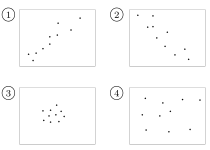
\includegraphics[keepaspectratio, width=50mm]{./mathclub-f/LV3_Q5.pdf}
    \end{minipage}
  \end{center}
\end{itembox}

Aの標準偏差は$\displaystyle\sqrt{\frac{11}{5}}$,Bの標準偏差は$\displaystyle\sqrt{\frac{44}{5}}$。
よって相関係数は,\\
\[\frac{4}{\sqrt{\frac{11}{5}}\cdot \sqrt{\frac{44}{5}}}=\frac{10}{11}\]
よって,相関係数が正で,正の相関があるため{\bfseries ①}が最も適する。\\


\subsection*{問6 セミナーハウス}
\begin{itembox}[l]{問題}
  KENKASHIの8文字を並べ変えたとき,2つのKが隣り合わない確率を求めよ。
\end{itembox}

文字の並べ方はそれぞれの文字を区別すると\( 8! \)通り\\
その中で,2つのKが隣り合う並べ方は$7!\cdot 2$通り\\
よって,求める確率は
\[1-\frac{7!\cdot 2}{8!}=\bm{\frac{3}{4}}\]


\subsection*{問7 体育館}
\begin{itembox}[l]{問題}
  下の図において,$ \mathrm{D}$ は$ \mathrm{BC}$ を$ 2:5$ に内分している。
  $ \mathrm{BD}=6$ のとき,$ \mathrm{EC}$ を求めよ。
  \begin{center}
    \begin{tikzpicture}[scale=0.16]
      \coordinate(A) at (23,12);
      \coordinate(B) at (14,0);
      \coordinate(C) at (35,0);
      \coordinate(D) at (20,0);
      \coordinate(E) at (0,0);
      \coordinate(Q) at (28,7);
      \draw[name path=tri](A)--(C)--(E)--cycle;
      \draw[name path=AB](A)--(B);
      \draw[name path=AD](A)--(D);
      \draw[name path=EQ](E)--(Q);
      \path[name intersections={of= EQ and AB, by={R}}];
      \draw[name path=CR](C)--(R);
      \draw[name path=BQ](B)--(Q);
      \path[name intersections={of= CR and AD, by={P}}];
      \draw(A)node[above]{A};
      \draw(B)node[below]{B};
      \draw(C)node[below right]{C};
      \draw(D)node[below]{D};
      \draw(E)node[below left]{E};
      \draw(P)node[below right]{P};
      \draw(Q)node[above right]{Q};
      \draw(R)node[above left]{R};
    \end{tikzpicture}
  \end{center}
\end{itembox}

チェバの定理より,\[\frac{\mathrm{BD}}{\mathrm{DC}}\times \frac{\mathrm{CQ}}{\mathrm{QA}}\times \frac{\mathrm{AR}}{\mathrm{RB}}=1\]
メネラウスの定理より,
\[ \frac{\mathrm{BE}}{\mathrm{EC}}\times \frac{\mathrm{CQ}}{\mathrm{QA}}\times \frac{\mathrm{AR}}{\mathrm{RB}}=1\]
よって,
\begin{align*}
  \frac{\mathrm{CQ}}{\mathrm{QA}}\times \frac{\mathrm{AR}}{\mathrm{RB}}&=\frac{5}{2}\\
  \frac{\mathrm{BE}}{\mathrm{EC}}&=\frac{2}{5}
\end{align*}
$\mathrm{BE}:\mathrm{EC}=2:5$より,$\mathrm{BC}=21$\\
よって,$\mathrm{BE}:\mathrm{EC}=2:5$なので,$\mathrm{EC}=\mathbf{35}$


\subsection*{問8 本部前}
\begin{itembox}[l]{問題}
  自然数 $ m, n\, (m\neq 10,\, n\neq 1)$ が
  \[ m^3+1^3=n^3+10^3\]
  を満たしているとき,$ m, n$ を求めよ。
\end{itembox}

因数分解して、999の約数から場合分けする方法もありますが、とっても簡単に解く方法(知識)があります。
詳しいエピソードは割愛します(タクシー数などと検索すれば分かると思います)が、$12^3+1=1729=10^3+9^3$と1729は2通りの立方の和で表される最小の数です。\\
これを知っていれば、すぐに$\bm{m=12,n=9}$と分かります。


\subsection*{問9 水道前}
\begin{itembox}[l]{問題}
  $x,y$を実数とするとき、$x^2+4xy+5y^2 -2y+3$の最小値を求めよ。
\end{itembox}

\[x^2+4xy+5y^2-2y+3={(x+2y)}^2+y^2-2y+3\]
このとき、$x=-2y$のときに最小値$y^2 -2y+3$をとることが分かります。
そのため、$y^2 -2y+3$の最小値を求めると、
\[y^2-2y+3={(y-1)}^2+2\]
よって、$y=1$のときに最小値{\bfseries 2}をとる。


\subsection*{問10 屋上入口}
\begin{itembox}[l]{問題}
  半径$a$の球に外接する正四面体の体積を求めよ。
\end{itembox}

\setcounter{equation}{0}
\begin{wrapfigure}[10]{r}{35mm}
  \begin{center}
    \tdplotsetmaincoords{70}{200}
    \begin{tikzpicture}[tdplot_main_coords,scale=0.5]
    
    \tikzmath{\a=1;}
    \tikzmath{\b=2*sqrt(6)*\a;}
    \coordinate (A) at ({\b/sqrt(3)},0,0);
    \coordinate (B) at ({-sqrt(3)*\b/6},{\b/2},0);
    \coordinate (C) at ({-sqrt(3)*\b/6},{-\b/2},0);
    \coordinate (O) at (0,0,{sqrt(6)*\b/3});
    \coordinate (H) at (0,0,0);
    \coordinate (M) at ({sqrt(3)*\b/12},{\b/4},0);

    \draw(A)node[left]{A};
    \draw(B)node[below]{B};
    \draw(C)node[right]{C};
    \draw(O)node[above]{O};
    \draw(H)node[below]{H};
    \draw(M)node[below left]{M};
    \draw(A)--(B)--(C)
    (A)--(O)--(B) (O)--(C);
    \draw[dashed](A)--(C);

    \draw[semithick](M)--(H)--(O) (A)--(H);
    \draw pic[draw=black, angle radius=0.2cm]{right angle=A--H--O};
    \draw pic[draw=black, angle radius=0.2cm]{right angle=A--M--H};
    \end{tikzpicture}
  \end{center}
\end{wrapfigure}
正四面体の一辺の長さを$b$とおく。
すると,各面は一辺が$b$の正三角形だから面積は,
\begin{align*}
  S&=b\times \frac{\sqrt{3}}{2}b \times \frac{1}{2}\\
  &=\frac{\sqrt{3}}{4}b^2
\end{align*}
右のようにH,Mをおくと,$\triangle\mathrm{AHM}$は3つの角が\ang{30}, \ang{60}, \ang{90}
の直角三角形だから,
\begin{align*}
  \mathrm{AH}&=\frac{b}{2}\times\frac{2}{\sqrt{3}}\\
  &=\frac{1}{\sqrt{3}}b
\end{align*}

\begin{wrapfigure}[12]{r}{60mm}
  \begin{center}
    \tdplotsetmaincoords{70}{200}
    \begin{tikzpicture}[tdplot_main_coords,scale=0.4]
    
    \tikzmath{\a=1;}
    \tikzmath{\b=2*sqrt(6)*\a;}
    \coordinate (I) at (0,0,{\a});
    \coordinate (A) at ({\b/sqrt(3)},0,0);
    \coordinate (B) at ({-sqrt(3)*\b/6},{\b/2},0);
    \coordinate (C) at ({-sqrt(3)*\b/6},{-\b/2},0);
    \coordinate (O) at (0,0,{sqrt(6)*\b/3});
    
    \draw(I)circle(\a cm);
    \fill(I)circle(2px);
    \draw(I)node[above left]{I};
    \draw(A)node[left]{A};
    \draw(B)node[below]{B};
    \draw(C)node[right]{C};
    \draw(O)node[above]{O};
    \draw(A)--(B)--(C)
    (A)--(O)--(B) (O)--(C);
    \draw[dashed](A)--(C);
    \end{tikzpicture}\\
    \tikz[->]{\draw(0,0.6)--(0,0.3)node[right]{\rlap{4つの三角錐に分ける}}--(0,0);}\\
    \minitet{A}{B}{C}+\minitet{O}{B}{A}\\+\minitet{O}{C}{B}+\minitet{O}{A}{C}
  \end{center}
\end{wrapfigure}
\noindent$\triangle\mathrm{AHO}$で三平方の定理を用いると,正四面体の高さは
\begin{align*}
  \mathrm{OH}^2&=\mathrm{OA}^2-\mathrm{AH}\\
  &=b^2-\frac{1}{3}b^2\\
  &=\frac{2}{3}b^2\\
  \mathrm{OH}&=\frac{\sqrt{6}}{3}b
\end{align*}
よって正四面体の体積は
\begin{equation}
  V=\frac{\sqrt{2}}{12}b^3\label{V1}
\end{equation}
また、図のように4つに分割して考えると、正四面体の体積は底面積$S$,高さ$a$の三角錐4つの体積に等しいから,
\begin{align}
  V&=\frac{\sqrt{3}}{4}b^2\times a\times \frac{1}{3}\times 4\notag\\
  &=\frac{\sqrt{3}}{3}ab^2\label{V2}
\end{align}
\eqref{V1}, \eqref{V2}を連立させて、体積は\qquad $\displaystyle\bm{8\sqrt{3}a^3}$


\subsection*{問11 徘徊者}
\begin{itembox}[l]{問題}
  $n^2$を120で割ると1余るような120以下の自然数$n$はいくつあるか。
\end{itembox}

\[n^2 = 120k+1 = 2^3\cdot 3\cdot 5k +1\:(\text{$k$は0以上の整数})\]
と表せる。
よって、$n^2$ を8, 3, 5で割るとそれぞれの余りが1であればよい。\\
$n^2$は奇数であるため、$n$も奇数である。\\
また、$n^2$は8で割り切れないので、$n^2$は4で割り切れない。\\
このとき、$n$が奇数ならば$n^2$を8で割ると1余る(証明略)。\\
ここで、奇数かつ3で割ると1余る数を考えると、
\[n=6a+1,\:6a+5\:(\text{$a$は整数})\]
と表せる。
また、$5$で割って$1$余る数を考えると、
\[n=5b+1,\:5b+4\:(\text{$b$は整数})\]
と表せる。
$n=6a+1$のとき、$n=5a+ (a+1)$なので、
\[a+1=5c+1,\:5c+4\:(\text{$c$は0以上の整数})\]
よって、\qquad $n=30c+1,\:30c+19$\\
$n=6a+5$のとき、$n=5(a+1)+a$なので、\qquad$a=5c+1,\:5c+4$\\
よって、\qquad$n=30c+11,\:30c+29$\\
この4式のいずれかを満たせばよいので、$n$の個数は$4\times4=\mathbf{16}$個\\


\newpage
\section{数II・Bコース}
\subsection*{問1 物理室}
掲載していた問題内容に誤りがありました。以下は正しい問です。ご迷惑おかけしました。
\begin{itembox}[l]{問題}
$\displaystyle 0\leqq \theta <2\pi$のとき,$\displaystyle \tan \theta \geqq -2-\sqrt{3}$の範囲を以下の選択肢から選べ。
\begin{description}
  \item[①] $\displaystyle\dwide 0\leqq \theta < \frac{\pi}{2},\, \frac{17}{18}\pi \leqq \theta < \frac{3}{2}\pi,\, \frac{35}{18}\pi \leqq \theta < 2\pi $
  \item[②] $\displaystyle\dwide \frac{\pi}{2} < \theta \leqq \frac{23}{36}\pi ,\, \frac{3}{2}\pi < \theta \leqq \frac{59}{36}\pi $
  \item[③] $\displaystyle\dwide \frac{\pi}{2} < \theta \leqq \frac{17}{18}\pi ,\, \frac{3}{2}\pi < \theta \leqq \frac{35}{18}\pi $ 
  \item[④] $\displaystyle\dwide 0\leqq \theta < \frac{\pi}{2},\, \frac{7}{12}\pi \leqq \theta < \frac{3}{2}\pi,\, \frac{19}{12}\pi \leqq \theta < 2\pi $ 
\end{description}
\end{itembox}

\begin{wrapfigure}{r}{40mm}
  \begin{tikzpicture}
    \draw[->,>=stealth,semithick](-1.5,0)--(1.5,0)node[above]{$x$};
    \draw[->,>=stealth,semithick](0,-4)--(0,1.5)node[above]{$y$};
    \draw(0,0)node[below left]{O};
    \draw(0,1)node[above right]{1};
    \draw(0,-1)node[below left]{-1};
    \draw(1,0)node[below right]{1};
    \draw(-1,0)node[below left]{-1};
    \draw[dashed](0,{-2-sqrt(3)})node[left]{$-2-\sqrt{3}$}--(1,{-2-sqrt(3)});
    \draw[name path=x1](1,1.5)--(1,-4);
    \draw[name path=C1](0,0)circle(1);
    \begin{scope}\clip(-1.5,-4)rectangle(1.5,1.5);
    \draw[name path=L1, domain=-1.5:1.1]plot(\x, {(-2-sqrt(3))*\x});
    \draw[name path=L2, domain=-1.5:1.5]plot(\x,-1*\x);
    \path[name intersections={of= C1 and L1, by={mainA,mainB}}];
    \path[name intersections={of= C1 and L2, by={subA,subB}}];
    \end{scope}
    \fill[red](mainA)circle(1.5pt);
    \fill[red](mainB)circle(1.5pt);
    \draw[red,semithick](1,0)arc(0:90:1);
    \draw[red,semithick](mainA)arc(105:270:1);
    \draw[red,semithick](mainB)arc(285:360:1);
    \fill[red](1,0.04)circle(1.5pt);
    \filldraw[red, fill=white](1,-0.04)circle(1.5pt);
    \filldraw[red, fill=white](0,1)circle(1.5pt);
    \filldraw[red, fill=white](0,-1)circle(1.5pt);
    \draw[->,>=stealth](0.3,0)arc(0:135:0.3);
    \draw[->,>=stealth](0.25,0)arc(0:315:0.25);
    \draw(subA)node[left]{\tiny$\frac{3}{4}\pi$};
    \draw(subB)node[below]{\tiny$\frac{7}{4}\pi$};
  \end{tikzpicture}
  \vspace{-50mm}
\end{wrapfigure}
不等式の示す概形は右の図の赤色の部分のようになる。
②,③は$\displaystyle\dwide 0\leqq \theta \leqq \frac{\pi}{2}$の範囲を含んでいないため,不適。\\
①は$\displaystyle\dwide \frac{3}{4}\pi < \frac{17}{18}\pi$より,不適。\\
よって正解は{\bfseries ④}


\newpage
\subsection*{問2 化学室}
\begin{itembox}[l]{問題}
  定義に従って,関数$f(x)=4x$の導関数を求めよ。
\end{itembox}

導関数の定義より,
\begin{align*}
  \lim_{h\to 0}\frac{4(x+h)-4x}{h}& = \lim_{h\to 0}\frac{4h}{h}\\
  &=\mathbf{4}
\end{align*}


\subsection*{問3 生物室}
\begin{itembox}[l]{問題}
  以下の数列の\Box に入る,最も適当な数を答えよ。%chktex 1
  \[2,\:\: 3,\:\:7,\:\:16,\:\:32,\:\: \Box ,\:\: 93,\:\: \cdots\]
\end{itembox}

この数列は階差数列$b_n$が$b_n=n^2$となっている。
よってもとの数列の第6項は,
\[32+5^2=\mathbf{57}\]


\subsection*{問4 特別棟4F}
\begin{itembox}[l]{問題}
  $a>-3$のとき,$\displaystyle\frac{a^3+6a+18}{a+3}$の最小値と,そのときの$a$の値を求めよ。
\end{itembox}

\begin{align*}
  \frac{a^3+6a+18}{a+3}&=\frac{{(a+3)}^2+9}{a+3}\\
  &=a+3+\frac{9}{a+3}
\end{align*}
相加平均・相乗平均の関係より,
\begin{align*}
  a+3+\frac{9}{a+3} &\geqq 2\sqrt{(a+3)\cdot \frac{9}{a+3}}\\
  a+3+\frac{9}{a+3} &\geqq 2\sqrt{9}\\
  a+3+\frac{9}{a+3} &\geqq 6
\end{align*}
最小値は$\displaystyle a+3=\frac{9}{a+3}$のときなので,%chktex 1
\begin{align*}
  a+3&=\frac{9}{a+3}\\
  {(a+3)}^2&=9\\
  a+3 &= \pm 3\\
  a &=0\quad (\because a>-3)
\end{align*}
よって,\qquad $\bm{a=0\text{\gtfamily のとき,最小値}6}$%chktex 1


\subsection*{問5 昇降口}
\begin{itembox}[l]{問題}
  $xy$平面上の3点$ (1,2), (2,1), (p,q)$の重心が$ (8,5)$のとき,$p$と$q$の和を求めよ。
\end{itembox}

重心の$x$座標は,
\begin{align*}
  \frac{1+2+p}{3}&=8\\
  p&=8\cdot 3-3=21
\end{align*}
重心の$y$座標は,
\begin{align*}
  \frac{2+1+q}{3}&=5\\
  q&=5\cdot 3-3=12
\end{align*}
よって\quad $p+q=21+12=\mathbf{33}$


\subsection*{問6 セミナーハウス}
\begin{itembox}[l]{問題}
  平行な2直線$4x-3y+3=0,\: 4x-3y-1=0$の距離を求めよ。
\end{itembox}

$4x-3y+3=0\cdots \text{①},\:4x-3y-1=0\cdots \text{②}$とおく。すると,%chktex 11
2直線の距離は①上の任意の点と②の直線の距離である。
①上の点を$ (0,1)$とすると,2直線の距離は
\[\frac{|4\cdot 0 - 3\cdot 1 -1|}{\sqrt{4^2+3^2}}=\frac{|-4|}{5}=\mathbf{\frac{4}{5}}\]


\subsection*{問7 体育館}
\begin{itembox}[l]{問題}
  $ \log_2 9,\, \log_4 3,\, \log_3 3,\, 0.4$ を小さい順に並べたとき,3番目に来るものを答えよ。
\end{itembox}

\begin{align*}
  \log_3 3=1\\
  \log_2 8=3\text{より,}\log_2 9 \geqq 3\\
  \log_4 4=1\text{より,}\log_4 3 \leqq 1\\
\end{align*}
よって3番目は\qquad$\bm{\log_3 3}$


\subsection*{問8 本部前}
\begin{itembox}[l]{問題}
  次の曲線と $ x$ 軸で囲まれた部分の面積を求めよ。
      \[ f(x)=x^2-6x\]
\end{itembox}

$f (x)=0$の解は,$x=0,6$,また,領域は$x$軸の下側にある。
よって面積は,
\begin{align*}
  -\int_0^6 (x^2-6x) dx&=-{\left[\frac{1}{3}x^3-\frac{6}{2}x^2\right]}_0^6\\
  &=-\left(\frac{1}{3}\cdot 6^3 - 3\cdot 6^2\right)\\
  &=-(72-108)\\
  &=\mathbf{36}
\end{align*}


\subsection*{問9 水道前}
\begin{itembox}[l]{問題}
  $ a_1 =1,\, a_2 =1,\, a_{n+2}=a_{n+1}+a_n\:\: (n=1,2,3,\ldots ) $で表される数列はどのような数列か。
\end{itembox}

\underline{答. フィボナッチ数列,Fibonacci series,美しい数列 など}
\subsubsection*{別解}
\setcounter{equation}{0}
特性方程式$x^2=x+1$の解$\displaystyle\dwide\frac{1+\sqrt{5}}{2},\frac{1-\sqrt{5}}{2}$を
それぞれ$\alpha,\beta$とすると,\[a_{n+2}-\alpha a_{n+1}=\beta(a_{n+1}-\alpha a_n)\]
となる。$a_{n+1}-\alpha a_n$は初項$a_2-\alpha a_1=1-\alpha$,公比$\beta$の等比数列だから,
\begin{align}
  a_{n+1}-\alpha a_n&=(1-\alpha)\beta^{n-1\notag}\\
  &=\beta^n \quad(\because 1-\alpha=\beta)\label{beta}
\end{align}
同様に$a_{n+2}-\beta a_{n+1}=\alpha(a_{n+1}-\beta a_n)$だから,
\begin{align}
  a_{n+1}-\beta a_{n}&=(1-\beta)\alpha^{n-1}\notag\\
  &=\alpha^n \quad(\because 1-\beta=\alpha)\label{alpha}
\end{align}
$\eqref{alpha}-\eqref{beta}$より,
\begin{align*}
  (\alpha-\beta)a_n&=\alpha^n-\beta^n\\
  a_n&=\frac{\alpha^n-\beta^n}{\alpha-\beta}
\end{align*}
よって,\qquad\textbf{一般項が$\displaystyle\dwide \bm{a_n=\frac{1}{\sqrt{5}}\left\{ {\left( \frac{1+\sqrt{5}}{2}\right)}^n - {\left( \frac{1-\sqrt{5}}{2}\right)}^n\right\}}$である数列。}


\subsection*{問10 屋上入口}
\begin{itembox}[l]{問題}
  関数 $f (x)=\sqrt[3]{3x+1}$ を微分せよ。
\end{itembox}

$y={(3x+1)}^{\frac{1}{3}},\: u=3x+1$とすると,
\begin{align*}
  \frac{dy}{dx}&=\frac{dy}{du}\cdot \frac{du}{dx}\\
  &=\frac{d}{du}\left(u^\frac{1}{3}\right)\cdot \frac{d}{dx}(3x+1)\\
  &=\frac{1}{3}u^{-\frac{2}{3}}\cdot 3\\
  &={(3x+1)}^{-\frac{2}{3}}\\
  &=\bm{\frac{1}{{(3x+1)}^{\frac{2}{3}}}}
\end{align*}


\newpage
\subsection*{問11 徘徊者}
\begin{itembox}[l]{問題}
  座標平面上で,$ x$ 座標,$ y$ 座標ともに整数である点を格子点という。
  座標平面上で,3つの不等式 $ y\geqq 0,\: y\leqq 3x,\: y\leqq -3x+12k$ ($ k$ は自然数)によって表される
  領域に含まれる格子点の個数を $ k$ を用いて表すと整数 $a,b,c$ を用いて$ ak^2 + bk + c$ となる。
  $a,b,c$ の和を求めよ。
\end{itembox}

\begin{wrapfigure}{r}{50mm}
  \begin{tikzpicture}[scale=0.5]
    \newcount\k
    \k=1
    \draw[->,>=stealth,semithick](-1,0)--(7,0)node[above]{$x$};
    \draw[->,>=stealth,semithick](0,-1)--(0,7)node[above]{$y$};
    \draw(0,0)node[below left]{O};
    \fill[pattern=north east lines, pattern color=red](0,0)--(2*\k ,6*\k )--(4*\k ,0)--cycle;
    \draw(0,0)--(2*\k ,6*\k )--(4*\k ,0)node[below]{$4k$}--cycle;
    \draw[dashed](2*\k ,6*\k)--($(0,-2)!(2*\k ,6*\k)!(0,7)$)node[left]{$6k$};
    \draw[dashed](2*\k ,6*\k)--($(-2,0)!(2*\k ,6*\k)!(7,0)$)node[below]{$2k$};
  \end{tikzpicture}
\end{wrapfigure}
3直線$y=0\cdots ①,\: y=3x\cdots ②,\\ y=-3x+12k\: (k\text{は自然数})\cdots ③$について,
①と②の交点の座標は$(0,0)$,①と③の交点の座標は$(4k,0)$,②と③の交点の座標は$(2k,6k)$であるから,
$ y\geqq 0,\: y\leqq 3x,\: y\leqq -3x+12k$によって表される領域$D$は,3点
$(0,0),(2k,6k),(4k,0)$を頂点とする三角形の周および内部である(右図の赤色部分で境界を含む)。

整数$j$が$0\leqq j \leqq 2k$を満たすとき,$D$に含まれる格子点座標が0以上$2k$以下である
点の個数$q$を$k$を用いて表すと
\begin{align*}
  q&=\sum_{j=0}^{2k} (3j+1)\\
  &=1+\sum_{j=1}^{2k} (3j+1)\\
  &=1+3\sum_{j=1}^{2k}j+\sum_{j=1}^{2k}1\\
  &=1+2\cdot \frac{1}{2}\cdot 2k(k+1)+2k\\
  &=6k^2+5k+1
\end{align*}
である。さらに,$D$に含まれる格子点で$x$座標が$(2k+1)$以上$4k$以下である点の個数を求めて$q$に加えれば,
$D$に含まれる格子点の数が求まる。直線$2k$に対して対称であることを利用すれば
\begin{align*}
  q&=q+\{q-(x=2k\text{上にある$D$に含まれる格子点個数})\}\\
  &=2q-\{(2k,0),(2k,1),\ldots ,(2k,6k)\text{の$6k+1$個}\}\\
  &=2\left(6k^2+5k+1\right)-(6k+1)\\
  &=12k+4k+1
\end{align*}
よって$a=12,b=4,c=1$なので,$a+b+c=\mathbf{17}$


\section{数III・Cコース}
\subsection*{問1 物理室}
\begin{itembox}[l]{問題}
  $ |\vec{\mathstrut a}|=2,\, | \vec{\mathstrut b} |=3,\, |\vec{\mathstrut a}+\vec{\mathstrut b}|=4 $ のとき,内積 $ \vec{\mathstrut a}\cdot \vec{\mathstrut b}$ の値を求めよ。
  %この問題だけレベルが3つくらい下です。解けてください!!
\end{itembox}

$|\vec{\mathstrut a}+\vec{\mathstrut b}|=4 $より,
\[|{\vec{\mathstrut a}}|^2+2\vec{\mathstrut a}\cdot \vec{\mathstrut b}+|\vec{\mathstrut b}|^2=16\]
$|\vec{\mathstrut a}|=2,|\vec{\mathstrut b}|=3$を代入して,
\begin{align*}
  2^2+2\vec{\mathstrut a}\cdot \vec{\mathstrut b} &= 16\\
  2\vec{\mathstrut a}\cdot \vec{\mathstrut b}&=3\\
  \text{よって}\quad \vec{\mathstrut a}\cdot \vec{\mathstrut b}&=\mathbf{\frac{3}{2}}
\end{align*}

\subsection*{問2 化学室}
\begin{itembox}[l]{問題}
  無限級数 $ \displaystyle \sum_{n=1}^{\infty} \frac{1}{n(n+3)}$ の和を求めよ。
  %2年でやるシグマに極限がついた問題。解けなきゃ困るよ
\end{itembox}
第$n$項までの部分和を$S$とすると,
\[S_n=\sum_{k=1}^{n}\frac{1}{k(k+3)}\]
これを計算して,
\[S_n=\frac{1}{3}\left( \frac{11}{6} - \frac{1}{n+1} -\frac{1}{n+2} -\frac{1}{n+3}\right)\]
よって,
\begin{align*}
  \lim_{n\to \infty} S_n&=\lim_{n\to \infty} \frac{1}{3}\left( \frac{11}{6} - \frac{1}{n+1} -\frac{1}{n+2} -\frac{1}{n+3}\right)\\
  &=\frac{1}{3}\cdot \frac{11}{6}=\frac{11}{18}
\end{align*}
よってこの無限級数の和は$\displaystyle\bm{\frac{11}{18}}$


\subsection*{問3 生物室}
\begin{itembox}[l]{問題}
  $ xy$ 平面上の楕円 $\displaystyle \frac{{(x+1)}^2}{3}+\frac{{(y-2)}^2}{4}=1$の焦点の座標を求めよ。
%楕円の基本 習ったのなら解けてほしい
\end{itembox}

楕円$\displaystyle\dwide \frac{{(x+1)}^2}{3}+\frac{{(y-2)}^2}{4}=1\: \cdots ①$は,楕円$\displaystyle \frac{x^2}{3}+\frac{y^2}{4}=1\: \cdots ②$を
$x$軸方向に$-1$,$y$軸方向に2だけ平行移動したものである。
$\sqrt{4 -3}=1$より,②の焦点の座標は
\[(0,1),(0,-1)\]
よって,①の焦点の座標は
\[\bm{(-1,3),(-1,1)}\]


\subsection*{問4 特別棟4F}
\begin{itembox}[l]{問題}
  行列 $A= \begin{pmatrix} 
    4 & 3 \\
    1 & 2 \\
  \end{pmatrix}$ に対して,$ A^2$ を$ pA+qE\, (p,q:\mbox{定数}) $ の形で表せ。
%定理さえ知っていれば解けるよ!
\end{itembox}

行列 $A= \begin{pmatrix} 
  4 & 3 \\
  1 & 2 \\
\end{pmatrix}$において,ケーリー・ハミルトンの定理より,
\begin{align*}
  A^2-(4+2)A+(4\cdot 2-3\cdot 1)E=0\\
  A^2-6A+5E=0
\end{align*}
よって,\qquad\underline{$A^2=6A-5E$}


\subsection*{問5 昇降口}
\begin{itembox}[l]{問題}
  $ \displaystyle \lim_{x\to -\infty} \left( \sqrt{x^2+x}+x\right) $を計算して♡
%「$x\to \infty $」に引っかからなければあとはふつう。計算はめんどくさいけどがんばれ!
\end{itembox}

$t=-x$とすると,$x=-t$であり,$x\to -\infty$のとき,$t\to\infty$だから,%chktex 1
\begin{align*}
  \lim_{x\to -\infty}\left( \sqrt{x^2+x}+x\right)&=\lim_{t\to \infty}\left( \sqrt{t^2-t}-t\right)\\
  &=\lim_{n\to\infty}\frac{\left(\sqrt{t^2-t}-t\right)\left(\sqrt{t^2-t}+t\right)}{\sqrt{t^2-t}+t}\\
  &=\lim_{n\to\infty}\frac{(t^2-t)-t^2}{\sqrt{t^2-t}+t}\\
  &=\lim_{n\to\infty}\frac{-t}{\sqrt{t^2-t}+t}\\
  &=\lim_{n\to\infty}\frac{-1}{\sqrt{1-\frac{1}{t}}+1}\\
  &=\frac{-1}{\sqrt{1}+1}=\bm{-\frac{1}{2}}
\end{align*}


\subsection*{問6 セミナーハウス}
\begin{itembox}[l]{問題}
  $ p$ を素数としたとき,$ 2p+1,\, 4p+1$ がいずれも素数であるような$ p$ の値をすべて求めよ。
\end{itembox}

$p$は素数であることから,2以上の整数である。
よって,$p$は正の整数$n$を用いて,$p=3n,\: p=3n+1,\: p=3n-1$のいずれかで表される。
\begin{itemize}
  \item $p=3n$のとき\\
    $p$が素数となるのは$n=1$のとき,つまり$p=3$のときのみである。
    このとき,$2p+1=7,\: 4p+1=13$はともに素数だから,条件を満たす。
  \item $p=3n+1$のとき\\
    $2p+1=2(3n+1)+1=3(2n+1)$と表され,$n\geqq 1$より$2n+1>1$だから,
    \(2p+1\) は3より大きい3の倍数で,素数ではない。\\
    よって,\(p=3n+1\) は条件を満たさない。
  \item \(p=3n-1\) のとき\\
    \(4p+1=4(3n-1)+1=3(4n-1)\) と表され,\(n\geqq 1\) より\( 4n-1>1\) だから,
    \(4n+1\) は3より大きい3の倍数で,素数ではない。\\
    よって,\(p=3n-1\) は条件を満たさない。
\end{itemize}
以上から,条件を満たす\(p\) の値は\(\bm{p=3}\) のみである。


\subsection*{問7 体育館}
\begin{itembox}[l]{問題}
  3円切手と8円切手がたくさんあります。これらを用いて作ることのできない金額は何種類あるか。
\end{itembox}

\( N\) を0以上の整数とする。
作りたい金額を \( N\) 円とすると,\( N\) は0以上の整数\( k\) を用いて
\( N=3k,\: 3k+1,\: 3k+2\) のいずれかで表すことができる。
\begin{itemize}
  \item \( N=3k\) のとき\\
    3円切手を\( k\) 枚使えば,すべての\( N\) をつくることができる。
  \item \( N=3k+1\) のとき\\
    \( k\geqq 5(N=16,19,22,\ldots)\) の場合は,3円切手\( (k-5)\) 枚と
    8円切手2枚を使えば,すべての\( N\) をつくることができる。\\
    \(k=0(\text{すなわち}N=1)\) の場合にはつくることができない。\\
    以下同様に,\( k=1(N=4),\: k=2(N=7),\: k=3(N=10),\: k=4(N=13)\) の場合もつくることができない。
  \item \( N=3k+2\) のとき\\
    \(k\geqq 2(N=8,11,14,\ldots)\) の場合は3円切手\( (k-2)\) 枚と8円切手1枚を使えば,すべての\( N\) をつくることができる。\\
    \(k=0(N=2),\: k=1(N=5)\) の場合はつくることができない。
\end{itemize}
以上から,つくることのできない金額は,1円,2円,4円,5円,7円,10円,13円\\
よって 個数は\quad \underline{7個}


\subsection*{問8 本部前}
\begin{itembox}[l]{問題}
  二次方程式 $ x^2+ax+b=0\, (a,b:\mbox{実数})$ の2つの解 $ \alpha , \beta $ が $ |\alpha |\leqq 1 $ かつ $|\beta |\leqq 1$ を
  満たすとき,点 $ (a,b)$ の存在範囲の領域の面積を求めよ。
\end{itembox}

与えられた方程式は実数係数の2次方程式あるから,
$\alpha ,\beta$は,ともに実数,ともに虚数のいずれかである。\\
(i) ともに実数の場合 判別式$D$について,
\[D=a^2-4\cdot 1\cdot b\geqq 0\: \text{より,}\: b\leqq\frac{1}{4}a^2\]
このとき,$-1\leqq x\leqq 1$で2つの解をもつ条件は,$f(x)=x^2+ax+b$について,
\begin{wrapfigure}[4]{r}{50mm}
  \begin{tikzpicture}[scale=0.8]
    \draw[->,>=stealth,semithick](-2,0)--(2,0)node[below]{$x$};
    \draw[dashed](0,-1)--(0,2)node[above right]{$f(x)=x^2+ax+b$};
    \begin{scope}\clip(-2,-1)rectangle(2,2);
      \draw[thick]plot[domain=-2:2](\x, {\x*\x-0.5});
    \end{scope}
    \draw[dashed](-1,0.5)--(-1,0)node[below]{$-1$};
    \draw[dashed](1,0.5)--(1,0)node[below]{$1$};
  \end{tikzpicture}
\end{wrapfigure}
\begin{align*}
  &-1\leqq -\frac{a}{2}\leqq 1,\\
  &\qquad 2\geqq a \geqq -2\\
  &f(1)=1+a+b\geqq 0,\\
  &\qquad b\geqq -a-1\\
  &f(-1)=1-a+b\geqq 0,\\
  &\qquad b\geqq a-1
\end{align*}

\begin{wrapfigure}[3]{r}{50mm}
  \begin{tikzpicture}[scale=0.4]
    \draw[->,>=stealth,semithick](-4,0)--(4,0)node[below]{$a$};
    \draw[->,>=stealth,semithick](0,-2)--(0,6)node[left]{$b$};
    \draw(0,0)node[above right]{O};
    \begin{scope}\clip(-4,-2)rectangle(4,6);
      \draw[thick]plot[domain=-4:4](\x, {\x*\x*0.25});
      \draw[thick]plot(\x, {-\x-1});
      \draw[thick]plot(\x, {\x-1});
    \end{scope}
    \fill[pattern=north west lines]plot[domain=-2:2](\x, {\x*\x*0.25})--(2,1)--(0,-1)--(-2,1);
    \draw[dashed](-2,0)node[below]{$-2$}--(-2,1)--(0,1)node[above left]{1}--(2,1)--(2,0)node[below]{$-2$};
    \draw(0,-1)node[right]{$-1$};
    \draw(-2,-2)node[below]{$b=a-1$};
    \draw(2,-2)node[below]{$b=-a-1$};
    \draw(3.5,{9/4})node[above left]{$\displaystyle b=\frac{1}{4}a^2$};
  \end{tikzpicture}
\end{wrapfigure}
\begin{align*}
  \text{したがって},
  \begin{cases}
    \displaystyle \dwide b\leqq \frac{1}{4}a^2\\
    -2\leqq a\leqq 2\\
    b\geqq -a-1\\
    b\geqq a-1
  \end{cases}
\end{align*}
\vspace{15mm}

(ii) ともに虚数の場合 判別式$D$について,
\[D=a^2-4\cdot 1\cdot b<0\text{より,}b>\frac{1}{4}a^2\]
このとき,虚数解$\alpha ,\beta$は共役複素数どうしであるから実数$p,q$を用いて,
$\alpha =p+qi$,$\beta=p-qi$と表せる。すると,
\[|\alpha |=|\beta |=\sqrt{(p+qi)(p-qi)}=\sqrt{p^2+q^2}\leqq 1\]
\[p^2+q^2\leqq 1\]

\begin{wrapfigure}[4]{r}{40mm}
  \begin{tikzpicture}[scale=0.4]
    \draw[->,>=stealth,semithick](-4,0)--(4,0)node[below]{$a$};
    \draw[->,>=stealth,semithick](0,-1)--(0,5)node[left]{$b$};
    \draw(0,0)node[below right]{O};
    \begin{scope}\clip(-4,-1)rectangle(4,5);
      \draw[thick]plot[domain=-4:4](\x, {\x*\x*0.25});
      \draw[thick]plot(\x,1);
    \end{scope}
    \fill[pattern=north west lines]plot[domain=-2:2](\x,{\x*\x*0.25});
    \draw[dashed](-2,0)node[below]{$-2$}--(-2,1);
    \draw[dashed](2,0)node[below]{2}--(2,1);
    \draw(0,1)node[above left]{1};
    \draw(2.5,1)node[above right]{$b=1$};
    \draw(2.2,3)node[above]{$\displaystyle b=\frac{1}{4}a^2$};
  \end{tikzpicture}
\end{wrapfigure}
また,解と係数の関係から,
\begin{align*}
  \alpha \beta =&(p+qi)(p-qi)\\
  =&p^2+q^2=b\text{より,}\\
  &0\leqq b \leqq 1
\end{align*}
したがって,\qquad $\begin{cases}
  \displaystyle\dwide b>\frac{1}{4}a^2\\
  0\leqq b\leqq 1
\end{cases}$

\begin{wrapfigure}{r}{40mm}
  \vspace{-20mm}
  \begin{tikzpicture}[scale=0.6]
    \draw[->,>=stealth,semithick](-3,0)--(3,0)node[below]{$a$};
    \draw[->,>=stealth,semithick](0,-2)--(0,3)node[left]{$b$};
    \filldraw[thick, pattern=north west lines](-2,1)--(2,1)--(0,-1)node[below left]{$-1$}--cycle;
    \draw[dashed](-2,0)node[below]{$-2$}--(-2,1);
    \draw[dashed](2,0)node[below]{2}--(2,1);
    \draw(0,1)node[above left]{1};
    \draw(0,0)node[above left]{\floattxt{O}};
  \end{tikzpicture}
\end{wrapfigure}
\vspace{15mm}
よって, (i), また (ii)より,右の図の斜線部分で境界を含む。
よってこの領域の面積は,
\[\frac{1}{2}\cdot 4\cdot 2=\mathbf{4}\]



\subsection*{問9 水道前}
\begin{itembox}[l]{問題}
  方程式 $ x^3=k{(x+1)}^2$ が相異なる3つの実数解を持つような定数 $ k$ の値の範囲を求めよ。
\end{itembox}

  $x=-1$は方程式を満たさない。\\
  よって,$x\neq 1$のとき,方程式は\qquad $\displaystyle \frac{x^3}{{(x+1)}^2}=k$\\%chktex 1
  求める実数解の個数は,関数$\displaystyle\frac{x^3}{{(x+1)}^2}$のグラフと
  直線$y=k$との共有点の個数に等しい。\\
  \begin{wrapfigure}{r}{60mm}
    \vspace{-10mm}
    \begin{equation*}
      \begin{array}{c||c|c|c|c|c|c|c}%chktex 44
        \hline%chktex 44
        x&\cdots&-3&\cdots&-1&\cdots&0&\cdots\\ \hline%chktex 44
        f'(x)&+&0&-&\times&+&0&+\\ \hline%chktex 44
        f(x)&\nearrow&-\dfrac{27}{4}\dwide&\searrow &\times&\nearrow &0&\nearrow\\ \hline%chktex 44
      \end{array} 
    \end{equation*}
    \vspace{-10mm}
  \end{wrapfigure}
$\displaystyle f(x)=\frac{x^3}{{(x+1)}^2}\:(x\neq -1)$とおくと%chktex 1
\begin{align*}
  f'(x)&=\frac{3x^2{(x+1)}^2-x^3\cdot 2(x+1)}{{(x+1)}^4}\\
&=\frac{x^2(x+3)}{{(x+1)}^3}
\end{align*}
$f'(x)=0$とすると\qquad$x=-3,0$\\
$f(x)$の増減表は右のようになる。

\noindent
\begin{wrapfigure}{r}{40mm}
  \vspace{-25mm}
  \begin{tikzpicture}[scale=0.4]
    \draw[->,>=stealth,semithick](-5,0)--(5,0)node[below]{$x$};
    \draw[->,>=stealth,semithick](0,-7.5)--(0,3)node[left]{$y$};
    \draw(0,0)node[below right]{O};
    \begin{scope}\clip(-5,-7.5)rectangle(5,3);
    \draw[very thick] plot[samples=100](\x, {pow(\x,3)/pow({\x+1},2)});
    \end{scope}
    \draw[dashed](-3,0)node[above left]{$-3$}--(-3,{-27/4})--(0,{-27/4})node[right]{$\displaystyle -\frac{27}{4}$};
    \draw(-1,-7.5)--(-1,0)node[above left]{$-1$}--(-1,3);
    \draw(2,0.5)node[right]{$y=f(x)$};
  \end{tikzpicture}
  \vspace{-20mm}
\end{wrapfigure}
また\qquad $\displaystyle\lim_{x\to -1}f (x)=-\infty$\\
よって,$y=f (x)$のグラフは右の図のようになる。
直線$y=k$との共有点の個数を調べると,方程式$x^3=k{(x+1)}^2$が
相異なる3つの実数解を持つような$k$の値の範囲は \qquad $\displaystyle \dwide \bm{k<-\frac{27}{4}}$

\newpage
\subsection*{問10 屋上入口}
\begin{itembox}[l]{問題}
  連立不等式\(y\geqq x^2-2x,\: y\leqq x,\: x\leqq 2\)の表す領域を$x$軸の周りに1回転してできる立体の体積$V$を求めよ。
\end{itembox}
\begin{wrapfigure}{r}{40mm}
  \begin{tikzpicture}[scale=0.7]
    \draw[->,>=stealth,semithick](-2,0)--(4,0)node[below]{$x$};
    \draw[->,>=stealth,semithick](0,-2)--(0,4)node[left]{$y$};
    \draw(0,0)node[above left]{O\:};
    \begin{scope}\clip(0,-1)rectangle(2,0);
      \fill[pattern=north west lines, pattern color=red]plot(\x,{pow(\x,2)-2*\x});
    \end{scope}
    \fill[pattern=north west lines, pattern color=red](0,0)--(2,0)--(2,2);    
    \begin{scope}\clip(-2,-2)rectangle(4,4);
      \draw[very thick] plot[samples=100](\x, {pow(\x,2)-2*\x});
      \draw[very thick] plot(\x,\x);
    \end{scope}
    \draw(3,3)node[left]{$y=x$};
    \draw(1,-1.2)node[right]{$y=x^2-2x$};
    \draw[dashed](0,-1)node[below right]{$-1$}--(1,-1)--(1,0)node[below right]{\floattxt{1}};
    \draw[dashed](0,2)node[left]{2}--(2,2)--(2,0)node[above right]{\:2};
    \draw[->](3.5,0)arc[start angle=10, end angle=360, x radius=0.2, y radius=0.4];
  \end{tikzpicture}

  \begin{tikzpicture}[scale=0.7]
    \draw[->,>=stealth,semithick](-1.5,0)--(4.5,0)node[below]{$x$};
    \draw[->,>=stealth,semithick](0,-2.5)--(0,2.5)node[left]{$y$};
    \draw(0,0)node[below left]{O };

    \begin{scope}\clip(0,0)rectangle(1,1);
      \fill[pattern=north west lines, pattern color=red]plot(\x,{-pow(\x,2)+2*\x});
    \end{scope}
    \fill[pattern=north west lines, pattern color=red](0,0)--(2,0)--(2,2);

    \begin{scope}\clip(-1.5,-2.5)rectangle(4.5,2.5);
      \draw[very thick] plot[samples=100](\x, {pow(\x,2)-2*\x});
      \draw[very thick] plot[samples=100](\x, {-pow(\x,2)+2*\x});
      \draw[very thick] plot(\x,\x);
      \draw[very thick] plot(\x,{-\x});
    \end{scope}
    \draw(2.3,2.3)node[left]{$y=x$};
    \draw(2.6,1.7)node[right]{$y=x^2-2x$};
    \draw(0.6,-2.5)node[right]{$y=-x$};
    \draw(2.5,-1)node[right]{$y=-x^2+2x$};

    \draw[dashed](0,-1)node[below right]{$-1$}--(1,-1)--(1,0)node[below right]{1}--(1,1)--(0,1)node[left]{1\!};
    \draw[dashed](0,2)node[left]{2}--(2,2)--(2,0)node[above right]{\:2}--(2,-2)--(0,-2)node[left]{$-2$};
    \draw(2,2)--(2,-2);

    \draw[->](3.5,0)arc[start angle=10, end angle=360, x radius=0.2, y radius=0.4];
  \end{tikzpicture}
  \vspace{-70mm}
\end{wrapfigure}
連立不等式$y\geqq x^2,\: y\leqq x,\: x\leqq 2$の表す領域は
右の図の斜線部分である。\\
この部分の周りの回転体は,右下の図の斜線部分の回転体と同じである。したがって
\begin{align*}
  V&=\pi \int_0^1 {(-x^2+2x)}^2dx+\pi \int_1^2 x^2 dx\\
  &=\pi \int_0^1 (x^4-4x^3+4x^2)dx+\pi {\left[\frac{x^3}{3}\right]}_1^2\\
  &=\pi {\left[\frac{x^5}{5}-x^4+\frac{4}{3}x^3\right]}_0^1+\pi \left(\frac{8}{3}-\frac{1}{3}\right)\\
  &=\pi \left(\frac{1}{5}-1+\frac{4}{3}\right)+\frac{7}{3}\pi=\bm{\frac{43}{15}\pi}
\end{align*}
\vspace{20mm}


\subsection*{問11 徘徊者}
\begin{itembox}[l]{問題}
  \( \displaystyle \lim_{x\to \frac{\pi}{2}} \left( \sin x\right)^{\tan^2 x}\) の値を求めよ。
\end{itembox}
\begin{align*}
  \lim_{x\to \frac{\pi}{2}} \left( \sin x\right)^{\tan^2 x}
  &=\lim_{x\to \frac{\pi}{2}} {\left\{{(\sin^2 x)}^{\tan^2 x}\right\}}^{\frac{1}{2}}\\
  &=\lim_{x\to \frac{\pi}{2}} {\left\{ {(1-\cos^2 x)}^{\frac{\sin^2 x}{\cos^2 x}} \right\}}^{\frac{1}{2}}\\
  &=\lim_{x\to \frac{\pi}{2}} {\left\{ {(1-\cos^2 x)}^{\frac{1}{\cos^2 x}} \right\}}^{\frac{1}{2}(1-\cos^2 x)}
\end{align*}
ここで,\( \cos^2 x=t\) とおくと,
\begin{align*}
  &\lim_{x\to \frac{\pi}{2}} {\left\{ {(1-\cos^2 x)}^{\frac{1}{\cos^2 x}} \right\}}^{\frac{1}{2}(1-\cos^2 x)}\\
  =&\lim_{t\to 0}{\left\{ {(1-t)}^{\frac{1}{t}} \right\}}^{\frac{1}{2}(1-t)}\\
  =&{\left( \frac{1}{e}\right)}^{\frac{1}{2}}\\
  =&\bm{\frac{1}{\sqrt{e}}}
\end{align*}
\end{document}